% -----------------
% abnTeX2: Modelo de Trabalho Acadêmico (tese de doutorado, dissertação de
% mestrado e trabalhos monográficos em geral) em conformidade com 
% ABNT NBR 14724:2011: Informação e documentação - Trabalhos acadêmicos -
% Apresentação
% -----------------

\documentclass[
	% -- opções da classe memoir --
	12pt,                     % tamanho da fonte
	openright,                % capítulos começam em pág ímpar (insere página vazia caso preciso)
	oneside,                  % twoside para impressão em verso e anverso. Oposto a oneside
	a4paper,                  % tamanho do papel. 
  % -- opções da classe abntex2 --
	% chapter=TITLE,          % títulos de capítulos convertidos em letras maiúsculas
	% section=TITLE,          % títulos de seções convertidos em letras maiúsculas
	% subsection=TITLE,       % títulos de subseções convertidos em letras maiúsculas
	% subsubsection=TITLE,    % títulos de subsubseções convertidos em letras maiúsculas
  % -- opções do pacote babel --
	english,                  % idioma adicional para hifenização
	% french,                 % idioma adicional para hifenização
	% spanish,                % idioma adicional para hifenização
	brazil                    % o último idioma é o principal do documento
]{abntex2}

% --- 
% Pacotes básicos 
\usepackage{lmodern}          % Usa a fonte Latin Modern		
\usepackage[T1]{fontenc}      % Seleção de códigos de fonte.
\usepackage[utf8]{inputenc}   % Codificação do documento (conversão automática dos acentos)
\usepackage{lastpage}         % Usado pela Ficha catalográfica
\usepackage{indentfirst}      % Indenta o primeiro parágrafo de cada seção.
\usepackage{color}            % Controle das cores
\usepackage{graphicx}         % Inclusão de gráficos
\usepackage{microtype}        % para melhorias de justificação
\usepackage{colortbl}         % Colorir linhas de tabelas
\usepackage[portuges]{datetime2}
% \DTMlangsetup[portuges]{showdayofmonth=false}
		
% ---
% Pacotes adicionais, usados apenas no âmbito do Modelo Canônico do abnteX2
\usepackage{lipsum}                           % para geração de dummy text

% ---
% Pacotes de citações
\usepackage[brazilian,hyperpageref]{backref}  % Paginas com as citações na bibl
\usepackage[num]{abntex2cite}                 % Citações padrão ABNT

% --- 
% CONFIGURAÇÕES DE PACOTES

% Configurações do pacote backref
% Usado sem a opção hyperpageref de backref
\renewcommand{\backrefpagesname}{Citado na(s) página(s):~}

% Texto padrão antes do número das páginas
\renewcommand{\backref}{}

% Define os textos da citação
\renewcommand*{\backrefalt}[4]{
	\ifcase #1
		Nenhuma citação no texto.
	\or
		Citado na página #2.
	\else
		Citado #1 vezes nas páginas #2.
	\fi}

% ---
% Informações de dados para CAPA e FOLHA DE ROSTO

\titulo{Impacto das modulações do IEEE 802.15.4g na qualidade de comunicação em ambiente de Smart Building}
\autor{Felipe Ferreira Bezerra da Silva}
\local{Campina Grande}
\data{\the\year{}}
\orientador{Prof. Ruan Delgado Gomes, D.Sc.}
\newcommand{\instituto}{
  Instituto Federal de Educação, Ciência e Tecnologia\\
  da Paraíba - Campus Campina Grande\\
  Curso Superior de Tecnologia em Telemática
}
\tipotrabalho{Trabalho de conclusão de curso}
% O preambulo deve conter o tipo do trabalho, o objetivo, 
% o nome da instituição e a área de concentração 
\preambulo{Monografia apresentada à Coordenação do Curso Superior de Tecnologia em Telemática do IFPB - Campus Campina  Grande,  como  requisito  parcial para conclusão.}

\renewcommand{\imprimircapa}{
  \begin{capa}
    \center

    \begin{figure}
      \begin{center}
        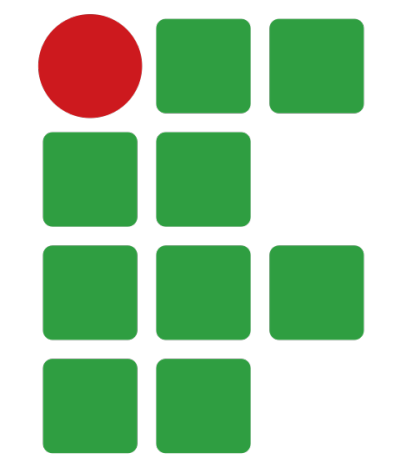
\includegraphics[width=1.8cm]{./assets/logo-ifpb.png}
      \end{center}
    \end{figure}

    \ABNTEXchapterfont \large \MakeUppercase{\instituto}

    \vspace*{2.5cm}

    \ABNTEXchapterfont \large \MakeUppercase{\imprimirautor}

    \vfill
    \begin{center}
      \ABNTEXchapterfont \bfseries \large \MakeUppercase{\imprimirtitulo}
    \end{center}
    \vfill
    % \vspace*{6.25cm}

    \large \imprimirlocal
    \par
    \large \imprimirdata
    \vspace*{1cm}
  \end{capa}
}


% ---
% Configurações de aparência do PDF final

\definecolor{blue}{RGB}{41,5,195}  % alterando o aspecto da cor azul

% informações do PDF
\makeatletter
\hypersetup{
  % pagebackref=true,
  pdftitle={\@title}, 
  pdfauthor={\@author},
  pdfsubject={\imprimirpreambulo},
  pdfcreator={LaTeX with abnTeX2},
  pdfkeywords={abnt}{latex}{abntex}{abntex2}{trabalho acadêmico}, 
  colorlinks=true,          % false: boxed links; true: colored links
  linkcolor=blue,           % color of internal links
  citecolor=blue,           % color of links to bibliography
  filecolor=magenta,        % color of file links
  urlcolor=blue,
  bookmarksdepth=4
}
\makeatother

% --- 
% Espaçamentos entre linhas e parágrafos 

\setlength{\parindent}{1.3cm} % O tamanho do parágrafo

% Controle do espaçamento entre um parágrafo e outro:
\setlength{\parskip}{0.2cm} % Tente também \onelineskip

\makeindex  % Compila o índice

\newcommand{\rd}[1]{{\color{green}[RD] #1}}
\newcommand{\ff}[1]{{\color{red}[FF] #1}}
\newcommand{\refact}[1]{{\color{red}[refatorar] #1}}

\citebrackets[] % fazer com que as citações dentro do texto virem colchetes

% ---
% Início do documento
\begin{document}
\frenchspacing  % Retira espaço extra obsoleto entre as frases.

% ---
% ELEMENTOS PRÉ-TEXTUAIS
% ---
\pretextual
% \imprimircapa
% \imprimirfolhaderosto*

% % Isto é um exemplo de Ficha Catalográfica, ou ``Dados internacionais de
% catalogação-na-publicação''. Você pode utilizar este modelo como referência. 
% Porém, provavelmente a biblioteca da sua universidade lhe fornecerá um PDF
% com a ficha catalográfica definitiva após a defesa do trabalho. Quando estiver
% com o documento, salve-o como PDF no diretório do seu projeto e substitua todo
% o conteúdo de implementação deste arquivo pelo comando abaixo:
%
% \begin{fichacatalografica}
%     \includepdf{fig_ficha_catalografica.pdf}
% \end{fichacatalografica}

\begin{fichacatalografica}
  \vspace*{\fill}                 % Posição vertical
  \hrule                          % Linha horizontal
  \begin{center}                  % Minipage Centralizado
    \begin{minipage}[c]{12.5cm}   % Largura

      \imprimirautor

      \hspace{0.5cm} \imprimirtitulo  / \imprimirautor. --
      \imprimirlocal, \imprimirdata-

      \hspace{0.5cm} \pageref{LastPage} p. : il. (algumas color.) ; 30 cm.\\

      \hspace{0.5cm} \imprimirorientadorRotulo~\imprimirorientador\\

      \hspace{0.5cm}
      \parbox[t]{\textwidth}{\imprimirtipotrabalho~--~\imprimirinstituicao,
        \imprimirdata.}\\

      \hspace{0.5cm}
      1. Palavra-chave1.
      2. Palavra-chave2.
      I. Orientador.
      II. Universidade xxx.
      III. Faculdade de xxx.
      IV. Título\\

      \hspace{8.75cm} CDU 02:141:005.7\\

    \end{minipage}
  \end{center}
  \hrule
\end{fichacatalografica}
       % Ficha bibliográfica
% \begin{errata}
  Elemento opcional da \citeonline[4.2.1.2]{NBR14724:2011}. Exemplo:

  \vspace{\onelineskip}

  FERRIGNO, C. R. A. \textbf{Tratamento de neoplasias ósseas apendiculares com
  reimplantação de enxerto ósseo autólogo autoclavado associado ao plasma
  rico em plaquetas}: estudo crítico na cirurgia de preservação de membro em
  cães. 2011. 128 f. Tese (Livre-Docência) - Faculdade de Medicina Veterinária e
  Zootecnia, Universidade de São Paulo, São Paulo, 2011.

  \begin{table}[htb]
    \center
    \footnotesize
    \begin{tabular}{|p{1.4cm}|p{1cm}|p{3cm}|p{3cm}|}
      \hline
      \textbf{Folha} & \textbf{Linha} & \textbf{Onde se lê} & \textbf{Leia-se} \\
      \hline
      1              & 10             & auto-conclavo       & autoconclavo     \\
      \hline
    \end{tabular}
  \end{table}

\end{errata}
        % Errata
% % Isto é um exemplo de Folha de aprovação, elemento obrigatório da NBR
% 14724/2011 (seção 4.2.1.3). Você pode utilizar este modelo até a aprovação
% do trabalho. Após isso, substitua todo o conteúdo deste arquivo por uma
% imagem da página assinada pela banca com o comando abaixo:
%
% \includepdf{folhadeaprovacao_final.pdf}
%

\begin{folhadeaprovacao}
  \begin{center}
    {\ABNTEXchapterfont\large\imprimirautor}

    \vspace*{\fill}\vspace*{\fill}
    \begin{center}
      \ABNTEXchapterfont \bfseries \Large \imprimirtitulo
    \end{center}
    \vspace*{\fill}

    \hspace{.45\textwidth}
    \begin{minipage}{.5\textwidth}
      \imprimirpreambulo
    \end{minipage}
    \vspace*{\fill}

    % Trabalho aprovado. \imprimirlocal, \today:
  \end{center}

  \assinatura{\textbf{\imprimirorientador} \\ Orientador}
  \assinatura{\textbf{Professor} \\ Bruno Jácome Cavalcanti, D.Sc.}
  \assinatura{\textbf{Professor} \\ Jerônimo Silva Rocha, D.Sc.}
  %\assinatura{\textbf{Professor} \\ Convidado 3}
  %\assinatura{\textbf{Professor} \\ Convidado 4}

  \begin{center}
    \vspace*{0.5cm}
    {\large\imprimirlocal}
    \par
    {\large\imprimirdata}
    \vspace*{1cm}
  \end{center}

\end{folhadeaprovacao}
      % Folha de aprovação
% \begin{dedicatoria}
  \vspace*{\fill}
  \centering
  \noindent
  \textit{ Este trabalho é dedicado às crianças adultas que,\\
    quando pequenas, sonharam em se tornar cientistas.} \vspace*{\fill}
\end{dedicatoria}
    % Dedicatória
% \begin{agradecimentos}
  Os agradecimentos principais são direcionados à Gerald Weber, Miguel Frasson,
  Leslie H. Watter, Bruno Parente Lima, Flávio de Vasconcellos Corrêa, Otavio Real
  Salvador, Renato Machnievscz\footnote{Os nomes dos integrantes do primeiro
    projeto abn\TeX\ foram extraídos de
    \url{http://codigolivre.org.br/projects/abntex/}} e todos aqueles que
  contribuíram para que a produção de trabalhos acadêmicos conforme
  as normas ABNT com \LaTeX\ fosse possível.

  Agradecimentos especiais são direcionados ao Centro de Pesquisa em Arquitetura
  da Informação\footnote{\url{http://www.cpai.unb.br/}} da Universidade de
  Brasília (CPAI), ao grupo de usuários
  \emph{latex-br}\footnote{\url{http://groups.google.com/group/latex-br}} e aos
  novos voluntários do grupo
  \emph{\abnTeX}\footnote{\url{http://groups.google.com/group/abntex2} e
    \url{http://abntex2.googlecode.com/}}~que contribuíram e que ainda
  contribuirão para a evolução do \abnTeX.

\end{agradecimentos}
        % Agradecimentos
% \begin{epigrafe}
  \vspace*{\fill}
  \begin{flushright}
    \textit{``Não vos amoldeis às estruturas deste mundo, \\
      mas transformai-vos pela renovação da mente, \\
      a fim de distinguir qual é a vontade de Deus: \\
      o que é bom, o que Lhe é agradável, o que é perfeito.\\
      (Bíblia Sagrada, Romanos 12, 2)}
  \end{flushright}
\end{epigrafe}
      % Epígrafe
% % resumo em português
\setlength{\absparsep}{18pt} % ajusta o espaçamento dos parágrafos do resumo
\begin{resumo}
  A Internet das Coisas possibilita uma forma de registrar nos mínimos detalhes tudo ao seu redor, como variações de temperatura em locais de uma cidade, bem como predizer se uma pessoa pode ou não ter problemas cardíacos a partir de sensores em seu corpo. A comunicação via rádio é uma solução para a implementação de sistemas IoT, porém este tipo de comunicação apresenta diversos desafios intrínsecos à sua utilização. Este trabalho se propõe a extender trabalhos anteriores, realizados em ambientes industriais e averiguar como a tecnologia de comunicação sem fio IEEE 802.15.4g Wi-SUN age em um ambiente predial, tendo em vista os diversos problemas que este tipo de ambiente causa em propagação de sinais de rádio. Para analisar, experimentalmente, o comportamento da tecnologia, foi implementada uma rede sem fio, na qual os dispositivos realizam cerca de 540 transmissões por hora, e os dados de suas transmissões foram armazenados e utilizados para analisar o desempenho da rede, a partir de parâmetros como taxa de entrega de pacotes e intensidade do sinal recebido. Como principal contribuição, este trabalho apresenta uma avaliação, em um ambiente real, do padrão IEEE 802.15.4g, mostrando como as particularidades das diferentes modulações são afetadas no ambiente predial. Como contribuição adicional, este trabalho cria e disponibiliza um conjunto de dados que podem ser utilizados por outros pesquisadores a fim de estudar e implementar técnicas de diversidade de modulação, possibilitadas graças aos diferentes esquemas de modulação disponíveis no 802.15.4g Wi-SUN.


  \textbf{Palavras-chaves}: IEEE 802.15.4g Wi-SUN. Redes Sem Fio. Internet das Coisas.
\end{resumo}

% resumo em inglês
\begin{resumo}[Abstract]
  \begin{otherlanguage*}{english}
    The Internet of Things provides a way to record everything around you in the smallest details, like the temperature variations in city locations, as well as predict whether or not a person may or may not have heart problems from sensors in their body. Radio communication is a solution for the implementation of IoT systems, however this type of communication presents several intrinsic challenges to its use. This work proposes to extend previous works, carried out in industrial environments, and to find out how the IEEE 802.15.4g Wi-SUN wireless communication technology acts in a building environment, considering the various problems that this type of environment causes in propagation radio signals. To analyze the behavior of the technology, a wireless network was implemented, in which the devices perform about 540 transmissions per hour, and the data of their transmissions were stored and used to analyze the performance of the network, using parameters such as  Packet Delivery Rate and Received Signal Strength Indication. As a main contribution, this work presents an assessment, in a real environment, of the IEEE 802.15.4g standard, showing how the particularities of the different modulations are affected in the building environment. As an additional contribution, this work creates and makes available a dataset that can be used by other researchers in order to study and implement modulation diversity techniques, made possible thanks to the different modulation schemes available in 802.15.4g Wi-SUN.


    \vspace{\onelineskip}

    \noindent
    \textbf{Key-words}: IEEE 802.15.4g Wi-SUN. Wireless Networks. Internet of Things.
  \end{otherlanguage*}
\end{resumo}

% resumo em francês 
% \begin{resumo}[Résumé]
%   \begin{otherlanguage*}{french}
%     Il s'agit d'un résumé en français.

%     \textbf{Mots-clés}: latex. abntex. publication de textes.
%   \end{otherlanguage*}
% \end{resumo}

% % resumo em espanhol
% \begin{resumo}[Resumen]
%   \begin{otherlanguage*}{spanish}
%     Este es el resumen en español.

%     \textbf{Palabras clave}: latex. abntex. publicación de textos.
%   \end{otherlanguage*}
% \end{resumo}
     % Resumos
% % ---
% Lista de ilustrações
\pdfbookmark[0]{\listfigurename}{lof}
\listoffigures*
\cleardoublepage

% ---
% Lista de tabelas
\pdfbookmark[0]{\listtablename}{lot}
\listoftables*
\cleardoublepage

% ---
% Lista de abreviaturas e siglas
\begin{siglas}
  \item[ABNT] Associação Brasileira de Normas Técnicas
  \item[abnTeX] ABsurdas Normas para TeX
\end{siglas}

% ---
% Lista de símbolos
\begin{simbolos}
  \item[$ \Gamma $] Letra grega Gama
  \item[$ \Lambda $] Lambda
  \item[$ \zeta $] Letra grega minúscula zeta
  \item[$ \in $] Pertence
\end{simbolos}
         % Listas

% ---
% Sumario
\pdfbookmark[0]{\contentsname}{toc}
\tableofcontents*
\cleardoublepage

% ---
% ELEMENTOS TEXTUAIS
% ---
\textual

% ---
% Introdução (exemplo de capítulo sem numeração, mas presente no Sumário)
\chapter*[Introdução]{Introdução}
\addcontentsline{toc}{chapter}{Introdução}
% ---

IoT é um conceito que vem ganhado força ao longo dos anos, e isto só foi possível após anos de estudo, prototipação e desenvolvimento de várias tecnologias, padrões e protocolos. Sendo os principais pontos, a miniaturização de processadores e sensores; melhoramento de baterias e otimização do uso destas; definição de novos protocolos de rede; e aumento da robustez de protocolos de comunicação sem-fio.

A Internet das Coisas, mais conhecida pelo seu acrônimo em inglês IoT, foi cunhada pelo engenheiro britânico Kevin Ashton no final dos anos 1990 onde ele, trabalhando para a P\&G, pensou na possibilidade de que os produtos da empresa estivessem munidos de identificadores e capazes de estabelecer comunicação sem fio e se comunicando através da internet, que na época estava se estabelecendo, criando assim uma internet onde as coisas estivesse conectadas\cite{KA_IOT}. Fazendo então que os computadores fossem capazes de rastrear e identificar tudo, reduzindo desperdícios e custos e identificando no momento certo quando substituir ou reparar um produto\cite{lopezIOT}.

Atualmente há diversas aplicações de IoT, desde grandes implementações como cidades inteligentes como em \cite{sotres2017practical}, onde na cidade de Santander na Espanha é implantado por toda a cidade sensores para analisar a qualidade do ar dos habitantes. Até aplicações de saúde como em \cite{zhang2015remote}, onde é coletado e analisado em tempo real informações de pressão sanguínea e peso corporal do paciente então é aplicado conceitos de aprendizado de maquina para verificar a probabilidade do paciente ter um evento de insuficiência cardíaca.

Após o termo ser criado em 1999, foi necessário anos de evolução tecnológica para a atual popularidade do conceito. Por exemplo, a criação da plataforma de desenvolvimento de hardware aberta Arduino em 2005\cite{OC_ARDUINO}, tornou fácil o estudo e a prototipação de itens de baixo custo. \ff{adicionar exemplos como o IPv6, baterias e os protocolos de Sem Fio}

A implementação de uma aplicação IoT necessita de uma rede de nó sensores distribuídas geralmente conectadas a um ou mais nó central, também conhecido como gateway, que tem por finalidade encaminhar os dados coletados para processamento. Para tal implementação, existem duas abordagens clássicas, conexões cabeadas entre os nós sensores e a utilização de redes sem fio\cite{gomes2017estimaccao}. Em vantagem a redes sem fio, as conexões cabeadas apresentam maior confiabilidade nas camada física. Porém, a utilização de redes sem fio se destaca, em relação a redes cabeadas, nos quesitos de flexibilidade, custo de implantação , facilidade e rápida de implementação e de manutenção\cite{gungor2009industrial}.

As vantagens que estas Redes de Sensores Sem Fio, também conhecidas como RSSF, apresentam então fazem elas se destacar, porém apresentam ainda desafios para uma implementação robusta. Pois o meio onde ocorre a comunicação via rádio é intrinsecamente não confiável, pode apresenta interferências, possui ruídos e alguns outros problemas clássicos de comunicação sem fio como sombreamento e propagação por multi percurso. Além de apresentar baixa taxa de transferência e valores de latência alto\cite{gomes2017estimaccao}.

Para contornar os diversos problemas da comunicação sem fio padrões e tecnologias foram desenvolvidos. Em cenários industriais, são proeminentes o WirelessHart, tecnologia RSSFs baseada no padrão Hart\cite{WIHART} e o padrão ISA100.11a. Ambos padrões são baseados na camada física do padrão IEEE802.15.4, porém apresentam diferentes implementações de Controle de Acesso ao Meio\cite{gomes2017estimaccao}, MAC. Além do cenário industrial, o Zigbee é uma tecnologia de baixo consumo energético, baixas taxas de transferência e de baixo custo baseado no protocolo de redes sem fio IEEE802.15.4 que tem por objetivo aplicações de controle remoto e automação\cite{ergen2004zigbee}. 6LoWPAN é um protocolo definido na RFC6282 pela IETF que pretende distribuir endereços de IP versão 6 para dispositivos de RSSF, sendo o principal alvo dispositivos que tem tecnologias baseadas no IEEE802.15.4, facilitando assim a conexão destas redes à internet já que podem compartilhar os mesmos endereços IPv6\cite{olsson20146lowpan}. LoRa é uma tecnologia que utiliza uma técnica de modulação proprietária chamada Chirp Spread Spectrum, que permite uma melhor sensibilidade e uma largura de banda fixa em troca de uma menor taxa de transferência\cite{sinha2017survey}. NarrowBand-IoT é uma tecnologia integrada com o padrão de comunicações moveis LTE, porém simplificada para reduzir custos e complexidade dos dispositivos, minimizando consumo de bateria\cite{sinha2017survey}.

Ao padrão IEEE802.15.4, desde sua criação em 2003, vem sendo anexado emendas criando assim novas possibilidades de usos e tecnologias. Com a emenda de 2015 ao padrão foi definida três modulações para utilização na camada física e mudanças para a MAC\cite{chang2012ieee}. Como forma. Em \cite{tuset2020reliability} foi proposto o uso destas três modulações em conjunto para melhorar a qualidade das comunicações, a partir de uma maior taxa de entregas de pacotes. Este artigo foi realizado em um cenário industrial onde os desafios para a comunicação sem fio estão, principalmente, em interferências de fontes externas e propagação por multi caminho. Pensando em analisar os efeitos da propagação de ondas de rádio em outro cenário, este trabalho então se propõe a analisar a comunicação sem fio de dispositivos em um ambiente predial, que possui como maior fonte de problemas para a comunicação a falta de linha de visada. Estudando como cada modulação se comporta a partir da verificação da taxa de entrega de pacotes, PDR, em cada modulação.

% \chapter{Fundamentação Teórica}
\label{fundamentacao}
Na fundamentação deste trabalho, será abordado como é dado a categorização de redes de telecomunicação. Em seguida será apresentado alguns padrões e tecnologias de comunicação sem fio para dispositivos de baixa potência. E então, será apresentado parâmetros de comunicação sem fio, que foram utilizados neste projeto, para medição de eficacia e a eficiência de um enlace sem fio.

% eficacia é um booleano para dizer se algo funciona ou não
% eficiência é uma escala para medir % de funcionamento.

\section{Classificação de redes}
\label{classRedes}
Segundo Tanembaum em \cite{tanembaum2011}, redes de telecomunicação são classificadas, comumente, de acordo com sua escala de abrangência.
\subsection{Classificação de redes: escala de abrangência}

\subsubsection*{Redes Pessoais - PAN}
Redes de área pessoal, ou redes de alcance limitado, são redes, geralmente sem fio, utilizadas para conexão entre sistemas pessoais. Por exemplo conexão de um fone de ouvido a um smartphone utilizando o Bluetooth. Aplicações de redes PAN vão além de conexão de dispositivos sem fio como mouses, teclados e fone. Também são utilizados em Sistemas Monitoração de Saúde onde no paciente há dispositivos coletando e enviando dados para o smartphone.

\subsubsection*{Redes locais - LAN}
Redes de área local, são redes privadas contidas dentro de um prédio, casa ou escritório. É formada pela conexão de computadores em uma rede de tamanho restrito, normalmente conectando os computadores através de um comutador(switch) por meio de cabos de par trançado utilizando uma topologia estrela. Atualmente é comum a utilização do Wi-Fi para conexão de redes locais, conhecidas como WLAN.

\subsubsection*{Redes geograficamente distribuídas - WAN}
Redes de longa distâncias que abrangem uma grande área geográfica, também se refere a redes que conectam países ou continentes. Por exemplo a Rede Nacional de Ensino e Pesquisa(RNP) que conecta diversas instituições de ensino superior do Brasil.

\subsubsection*{Redes de loga distância com baixo consumo energético - LPWAN}
Dispositivos que implementam redes de baixo consumo energético ganharam popularidade na industria e nas comunidades de pesquisa pois podem estabelecer comunicação sem fio de longas distâncias, de 10 a 40 km em zonas rurais e 1 a 5 km em zonas urbanas com baterias que podem durar mais de 10 anos com uma única carga \cite{mekki2019comparative}. A utilização deste tipo de rede se tornou fundamental para a implementação de RSSFs, oferecendo confiabilidade e baixo custo de implantação e manutenção para redes sem fio. Abaixo serão apresentadas os principais padrões e tecnologias utilizadas.


\section{Padrões e tecnologias de comunicação para redes LPWAN}
\label{padrõesSF}
Segundo Tanembaum em \cite{tanembaum2011}, sem coordenação e cooperação entre as fabricantes de dispositivos haveria o caos completo onde não seria possível a interoperabilidade de sistemas. Sistemas IoT, como demonstrado em \cite{sotres2017practical}, podem ter apresentar sistemas diferentes com vários dispositivos. Portanto a padronização das telecomunicações são imprescindíveis atualmente. Permitindo dispositivos de diferentes fabricantes consigam se comunicar, não importando quem produziu a placa de rede, os cabos, roteadores ou comutadores.

\subsection{LoRa}
LoRa, abreviação para Long Range, é uma tecnologia que utiliza o padrão LoRaWAN e um protocolo de acesso ao meio de mesmo nome. Modula sinais sub-GHz na faixa ISM utilizando uma técnica de modulação  privada chamada Chirp Spread Spectrum. que espalha um sinal de banda curta por todo um canal de banda larga, esta técnica possibilita uma maior resistência a interferências e torna mais difícil detectar ou obstruir o canal de comunicação. A taxa de transferência pode variar de 300 bits/s a até 50 kbits/s, dependendo do fator de espalhamento utilizado na comunicação. O payload máximo de uma mensagem é 243 bytes \cite{mekki2019comparative}.

A tecnologia LoRa é desenvolvida pela empresa estadunidense SemTech e o padrão LoRaWAN é mantido pelo consorcio de empresas chamado LoRa Alliance.

\subsection{NB-IoT}
NarrowBand IoT é uma tecnologia especificada na versão 13 do 3GPP. Esta tecnologia opera na faixa de frequência celular(LTE e GSM), modulando os sinais utilizando a técnica QPSK. Utiliza faixas de frequência não ocupadas da faixa de frequência LTE. Seu protocolo é baseado em uma versão simplificada do protocolo LTE, que reduz as funcionalidades do LTE para melhor se adequar sua utilização para IoT, por exemplo, funções como monitoramento da qualidade do sinal ou conectividade dupla não são utilizadas, visando diminuir o uso de energia e aumentar a vida util da bateria. Possui taxa transferência máxima de 200 kbits/s e seu payload máximo é de 1600 bytes.

\subsection{SigFox}
SigFox é uma tecnologia que não possui padronização oficial e é mantida pela empresa de homônima. Os nós finais conectados a esta rede enviam para as estações radio-base mensagens utilizando a modulação BPSK utilizando bandas de frequência ultra-estreitas, até 100 Hz, na faixa de frequência ISM. Como utiliza uma faixa de frequência é bastante eficiente energeticamente e bastante resistente a interferência. Porém, não pode oferecer taxas de transferência acima de 100 bp/s.

A empresa SigFox oferece uma solução com conectividade ponta a ponta, o que significa que os dados entre o nó final são transmitidos para as estações rádio-base e vão diretamente para os servidores da empresa. Sendo possível apenas o envio de 140 mensagens por dia e cada mensagem enviada pode ter um payload máximo de 12 bytes.

\subsection{IEEE 802.15.4}
O padrão IEEE 802.15.4 define em seu texto, camadas físicas e de acesso ao meio utilizando a faixa ISM sub-GHz e 2.4 GHz, utilizando, respectivamente, as modulações BPSK e O-QPSK. Possuindo uma taxa de transferência máxima de 250 kbits/s utilizando a faixa de frequência de 2.4 GHz com um tamanho máximo de payload de 127 bytes \cite{munoz2018overview}\cite{gomes2017estimaccao}. Este padrão é utilizado como base para a utilização do ZigBee.

\subsection*{Emenda 'g'}
Em 2015 foi proposto uma revisão que incorpora uma novo esquema de modulações para permitir uma melhor volatilidade entre a faixa de comunicação, ocupação da largura de banda, taxa de transferência de dados e confiabilidade da comunicação para melhor se adequar com a aplicação. O padrão então foi adotado como uma emenda ao padrão de 2003, definindo assim o padrão IEEE 802.15.4g que incluia as modulações SUN(Redes de Utilidades Inteligentes, Smart Utility Network)\cite{tuset2020reliability}.
A seguir uma visão geral das modulações SUN de acordo apresentado em \cite{tuset2020reliability}:
\subsubsection*{FSK-SUN}
Foi incluída no padrão devido a sua eficiência e compatibilidade com sistemas legado. Possui 3 modos de operação para cada uma das faixas de frequência definidas no padrão e possui parâmetros de canal e de modulação, nos quais é possível definir o tipo de modulação, o espaçamento do canal e o índice de modulação. Estes parâmetros definem uma faixa de taxa de transferência de 50 kbits/s a até 50 kbits/s.
\subsubsection*{OQPSK-SUN}
Esta modulação está presente no texto original do padrão e foi estendida nesta emenda para adicionar bandas de frequência e suportar diferentes fatores de espalhamentos para conseguir atingir taxas de transferência entre 6.25 kbits/s a até 500 kbits/s.
\subsubsection*{OFDM-SUN}
Esta modulação consegue prover altas taxas de transferência e maiores faixas de comunicação, enquanto consegue lidar com interferência e propagação por multi-caminho. Utiliza diferentes Esquemas de Modulação e Codificação para alternar em modulações, como BPSK, QPSK e 16-QAM, e esquemas de repetição de frequência para prover uma faixa de taxa de transferência entre 50 kbits/s a até 800 kbits/s em um canal com a largura de banda que varia entre 200kHz e 1.2MHz.

\subsubsection*{Diversidade de Modulação}
Em \cite{gomes2020improving} os autores propõem a utilização das três modulações SUN em um esquema de diversidade de modulação como forma de aumentar a confiabilidade do enlace sem fio.

\section{Parâmetros do Enlace Sem Fio}
\label{paramSF}
Algumas métricas são utilizadas para medir a qualidade de um enlace sem fio, algumas estão mais relacionadas a camada física, como RSSI, e outras estão mais relacionadas a camada de aplicação como PDR. Estas serão melhor detalhadas abaixo.
\subsection*{RSSI}
Received Signal Strength Indicator, Indicador da Força do Sinal Recebido em tradução livre, é uma medida da energia total presente em um sinal de rádio recebido. RSSI é um valor relativo e pode variar de acordo com a fabricante do transceptor de rádio\cite{UNDERSTANDING_RSSI}. Geralmente o valor de RSSI é apresentado em números negativos que vão de -100 até 0, onde valores próximos de -100 são sinais de baixa qualidade e sinais com valores próximos a 0 são de ótima qualidade.

\subsection*{PDR}
Packed Delivery Ratio, Taxa de Entrega de Pacotes, é um indicador de camada de aplicação que relaciona a quantidade de pacotes recebidos pelo receptor pela quantidade de pacotes enviados pelo transmissor. O PDR pode ser um valor importante para medir um enlace de dados, pois dependendo da aplicação há uma taxa minima de entrega de pacotes, por exemplo, algumas aplicações industriais necessitam de um PDR superior a 99.9\%


\chapter{Experimento}
\label{experimento}

Nesta Seção é apresentado o experimento de implementação de uma RSSF em um ambiente de \emph{Smart Building}, utilizando a implementação do padrão IEEE 802.15.4g SUN dos dispositivos OpenMote-B \cite{tuset2020dataset}. A finalidade deste experimento é avaliar o desempenho da rede analisando valores de PDR e RSSI obtidos.

O experimento foi realizado em um dos prédios do campus Campina Grande do IFPB, Instituto Federal de Educação, Ciência e Tecnologia da Paraíba. Sendo este constituído principalmente de salas de escritório e de alguns laboratórios, possuindo 4 andares separados por pisos de concreto. Além desse cenário ser particularmente desafiador para um enlace sem fio pois não é possível ter uma linha de visada entre o transmissor, as paredes e pisos facilitam a ocorrência de propagação por múltiplos caminhos e a possibilidade áreas de sombreamentos de sinais.

\section{Visão Geral}
\label{subsec:visaogeral}
A rede foi composta por 11 dispositivos transmissores, denominado pelo restante do texto como Tx, que enviavam nove replicas de mensagens, três para cada modulação do padrão IEEE 802.15.4g SUN. Três receptores, denominado pelo restante do texto como Rx, foram configurados para receber mensagens em apenas uma das modulações do padrão. Os dispositivos Rx, conectados a um computador, enviavam as mensagens recebidas pelo rádio para a porta serial. O computador utiliza um sistema operacional baseado em GNU/Linux e executa um \emph{script Python} que lê as mensagens seriais enviadas pelos dispositivos Rx, estruturava e persistia no banco de dados InfluxDB. AFigura \ref{fig:rede_visão_geral} representa uma visão geral do funcionamento da rede.

\begin{figure}[h]
      \begin{center}
            \caption{Visão Geral da Rede.}
            \includegraphics[width=0.8\textwidth]{./sections/textual/chapters/images/rede_visão_geral.png}\\
            Fonte autoral.
            \label{fig:rede_visão_geral}
      \end{center}
\end{figure}

Os dispositivos Tx foram espalhados pelos quatro andares do prédio, posicionados em canaletas, como demonstrado naFigura \ref{fig:tx_canaleta}, e no interior de uma sala. Enquanto que os dispositivos Rx foram colocados no interior do laboratório GComPI, presente no primeiro piso do prédio.

\begin{figure}[h]
      \begin{center}
            \caption{Exemplo de Local dos Dispositivos Tx.}
            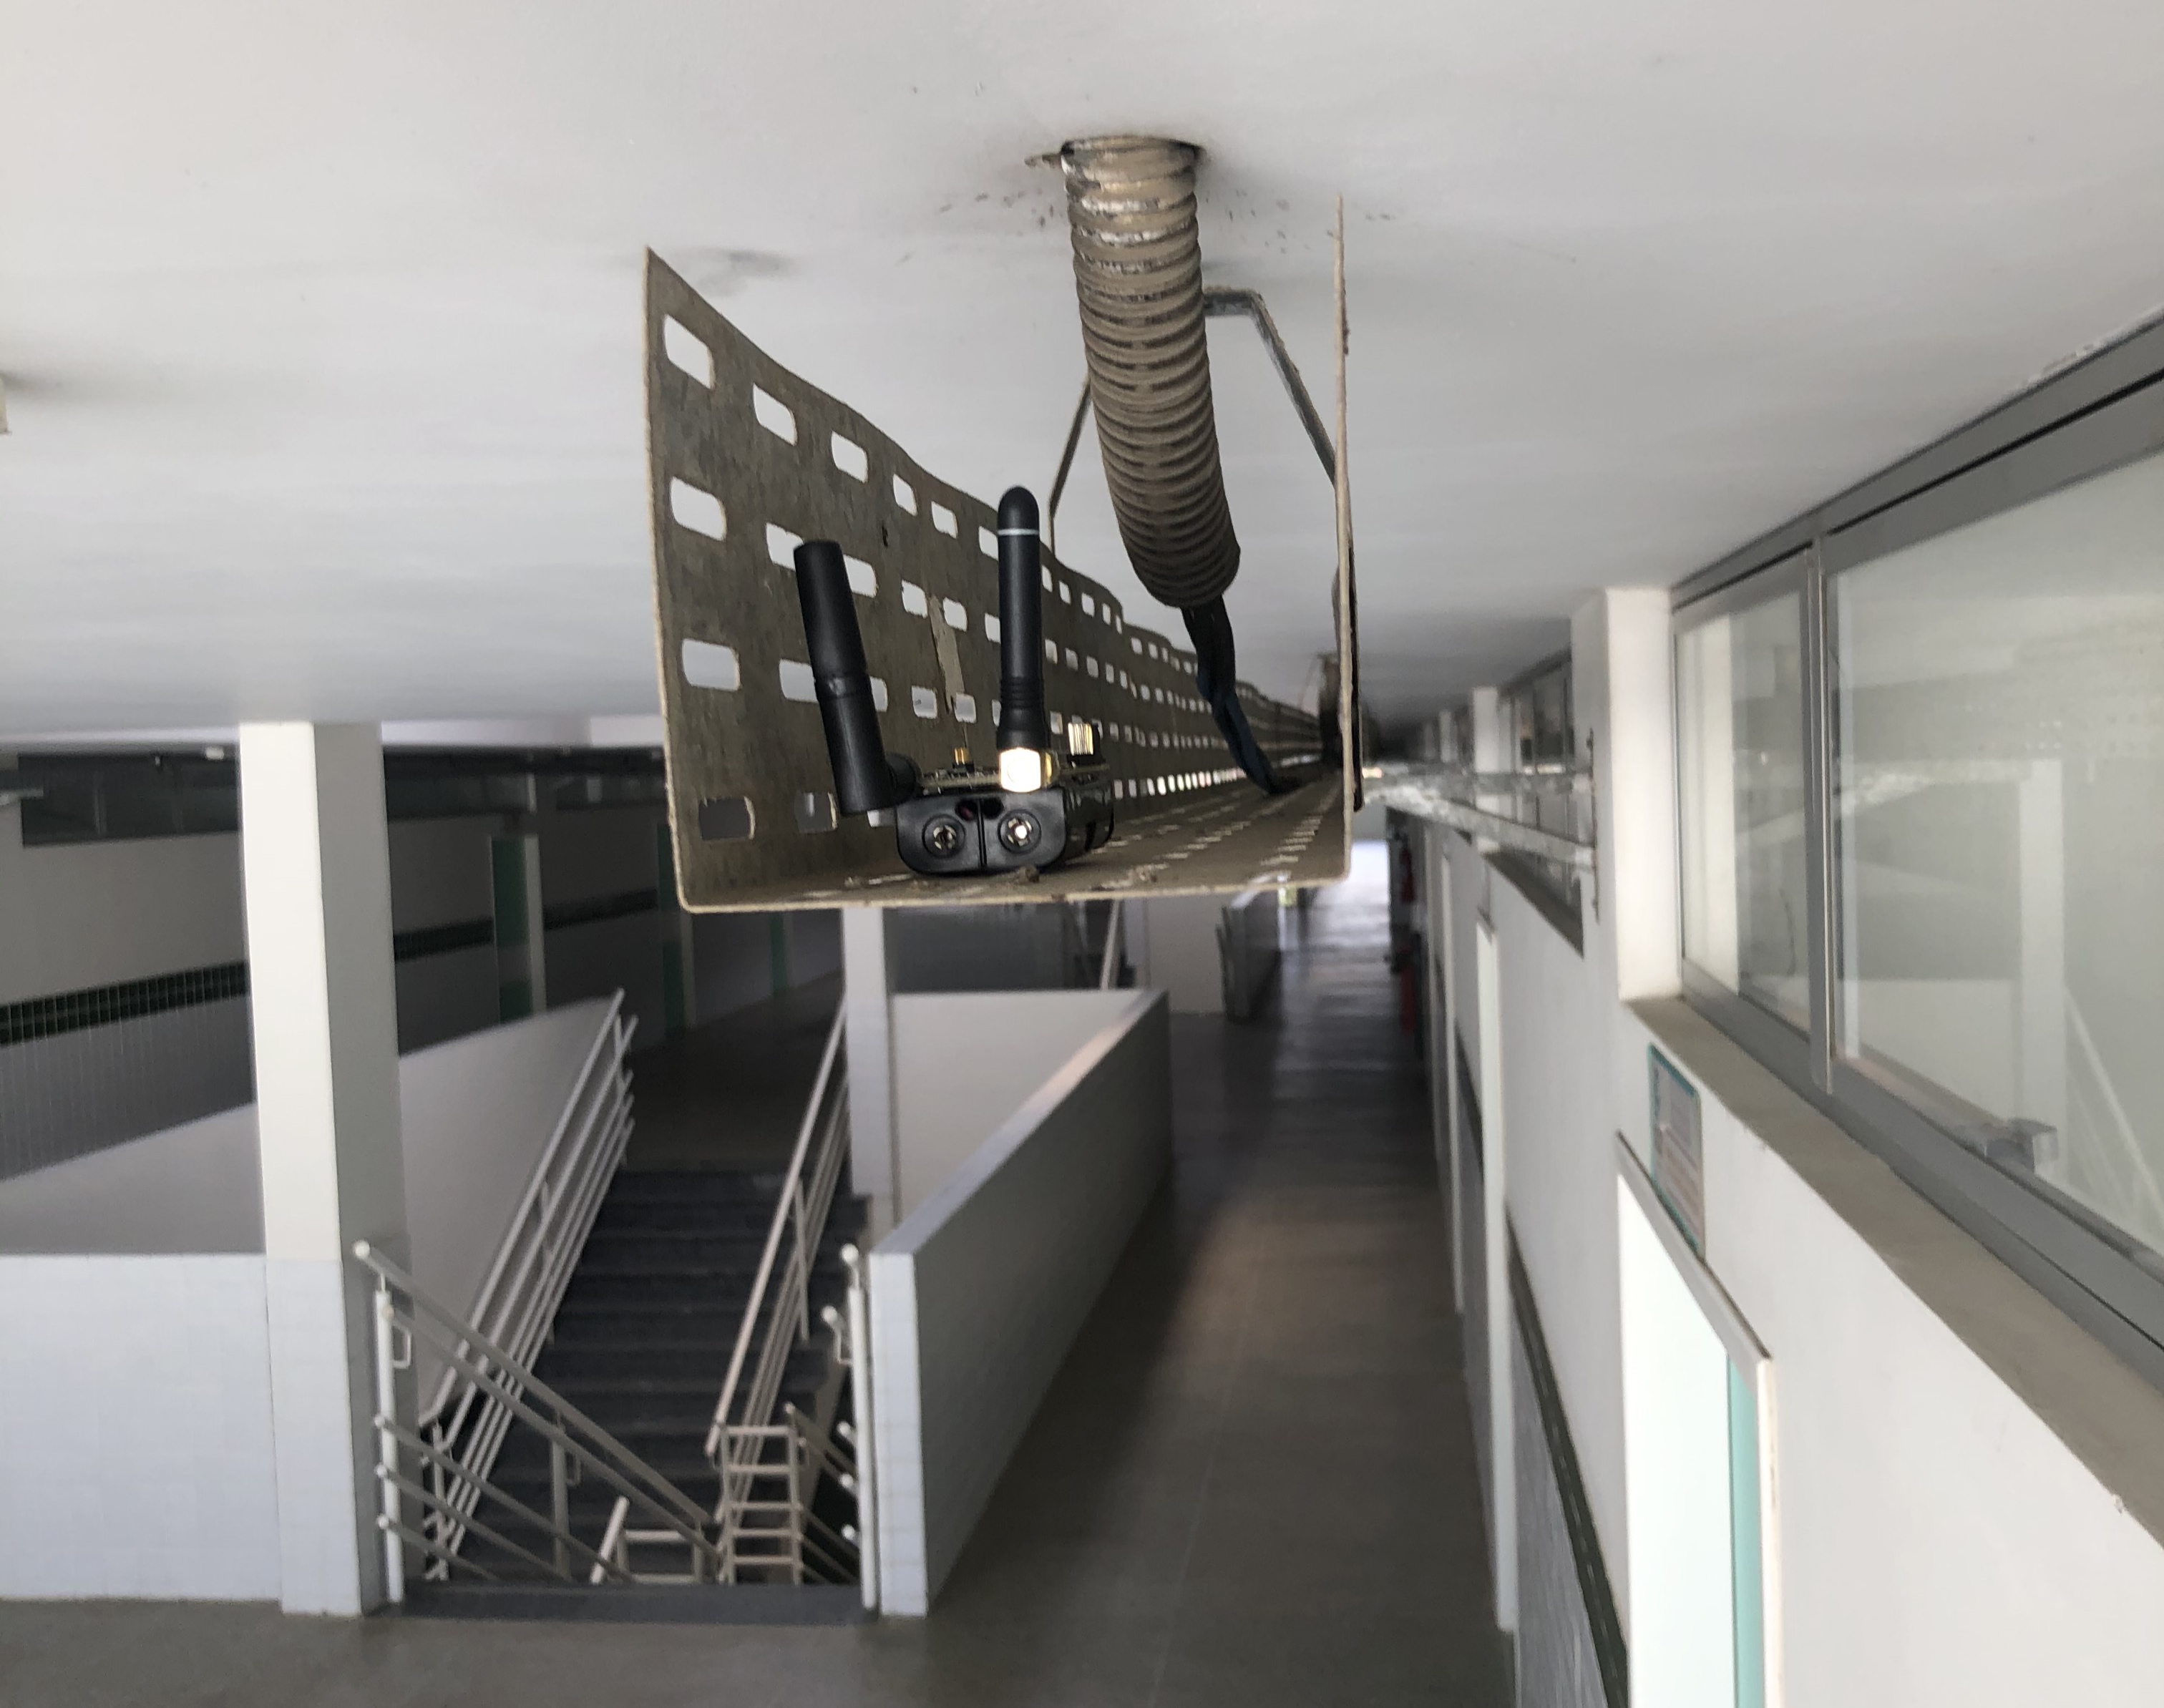
\includegraphics[width=10cm]{./sections/textual/chapters/images/tx_canaleta.jpg}\\
            Fonte autoral.
            \label{fig:tx_canaleta}
      \end{center}
\end{figure}

\section{OpenMote B}
O OpenMote B é um hardware de desenvolvimento e prototipação de plataformas IoT. Contém o processador SoC, \emph{System-on-Chip}(Sistema em um \emph{Chip}), CC2535 da Texas Instruments, constituído de um ARM Cortex-M3, com 32 K\emph{bytes} de memoria RAM e 512 K\emph{bytes} de memoria Flash. Embarcado neste processador, há um transceptor com suporte ao padrão IEEE 802.15.4 que utiliza a modulação DSSS-OQPSK na faixa ISM de 2,4GHz. Junto com o processador, o OpenMote B vem com um transceptor AT86RF215 da ATMEL que implementa as três modulações do padrão IEEE 802.15.4g nas faixas de frequência ISM abaixo das frequências de 1GHz e na faixa ISM 2,4GHz \cite{openmoteb-userguide}.

Para a realização do experimento, o código base do firmware dos dispositivos está presente no repositório \cite{openmoteb-firmware}. Foram realizadas alterações ao código base e estão disponíveis no repositório \cite{openmoteb-gcompi}.

\section{Transmissão dos dados}
Os dispositivos foram configurados para realizar, a cada minuto, três ciclos de envio de mensagens, como representado naFigura \ref{fig:ciclo_envio}, em cada ciclo são transmitidas três mensagens, uma para cada modulação do padrão. A cada envio de mensagem o dispositivo espera 50 ms. Entre cada ciclo de envio o dispositivo espera 100 ms, do primeiro para o segundo ciclo, e 200 ms, do segundo para o terceiro ciclo. Ao realizar os três ciclos de transmissão, o dispositivo entra em modo espera por 58250 ms totalizando assim 60 segundos para o envio de nove mensagens, cada transmissão, com uma carga útil de 32 \emph{bytes}, leva um total de 100 ms, para a taxa de transmissão de 50 k\emph{bit}/s.

\begin{figure}[h]
      \centering
      \caption{Ciclo de Envio de Mensagens.}
      
\includegraphics[width=\textwidth]{./sections/textual/chapters/images/metodo_ciclo_envio.png}\\
      Fonte autoral.
      \label{fig:ciclo_envio}
\end{figure}

Cada mensagem transmitida é constituída dos seguintes campos:
\begin{itemize}
      \label{table:estruturaTx}
      \item Identificador do dispositivo: um campo de 6 \emph{bytes} que registra uma letra entre ``a'' e ``k'' que identifica cada um dos onze dispositivos Tx;
      \item Identificador de pacote: um campo de 8 \emph{bytes} que registra um contador que é também a identificação do pacote;
      \item Identificador da modulação: um campo de 1 \emph{byte} que registra em qual modulação o pacote foi enviado;
      \item Identificador de Pacote do Transmissor: um campo de 1 \emph{byte} que registra em qual dos ciclos de transmissão, ciclo um, dois ou três, o pacote foi enviado;
      \item Quantidade de Tentativas do CSMA: um campo de 1 \emph{byte} que registra quantas vezes o transmissor sensoreou o canal de radiofrequência antes de realizar a transmissão, o valor pode ir de 1 até 3, caso chegue na terceira tentativa o dispositivo não realiza a transmissão;
      \item Valor de RSSI do transmissor: um campo de 1 \emph{byte} que registra o valor de energia do canal. Se o valor estiver acima do valor apresentado no campo ``Limiar do CCA'' na Tabela \ref{table:config} o dispositivo espera um tempo aleatório, em ms, e realiza outra tentativa de transmissão.
\end{itemize}

Para completar os 32 \emph{bytes} de carga útil cada mensagem foi preenchida com 14 \emph{bytes}.

% \begin{table}[h!]
%     \centering
%     \begin{tabular}{|c c c c|}
%         \hline
%         Valor       & slug & \makecell{Tamanho   \\ (\emph{bytes})} & Descrição                                                                                \\ [0.5ex]
%         \hline\hline
%         \makecell{Identificador                  \\ do dispositivo}           &      & 6                                          & Uma letra entre ``a'' e ``k''                                                            \\\hline
%         \makecell{Identificador                  \\ de pacote}                &      & 8                                          & Um número inteiro positivo                                                               \\\hline
%         \makecell{Identificador                  \\ da modulação}             &      & 1                                          & O número 1, 2 ou 3\footnote{Respectivamente as modulações SUN-FSK, SUN-OQPSK e SUN-OFDM} \\\hline
%         \makecell{Identificador                  \\ de Pacote do Transmissor} &      & 1                                          & \makecell{Em qual ciclo de envio foi transmitido\\(ciclo 1, 2 ou 3)}\\\hline
%         \makecell{Quantidade de                  \\ Tentativas do CSMA}       &      & 1                                          & \makecell{Número de tentativas do CSMA\\(máximo de 3 tentativas)}                                                \\\hline
%         \makecell{Valor de RSSI                  \\ do transmissor}           &      & 1                                          & \makecell{Quantidade de energia registrada\\no momento da transmissão}                                                                                        \\\hline
%         \makecell{} &      &                   & \\\hline                                                                                        \\ \hline
%         \hline
%     \end{tabular}
%     \caption{Configurações utilizadas de cada modulação.}
%     \label{table:estruturaTx}
% \end{table}

Na Tabela \ref{table:config} estão descritas as configurações de operação de cada modulação.
\begin{table}[h!]
      \centering
      \begin{tabular}{|c c c c|}
            \hline
            Modulação & SUN-FSK & SUN-OQPSK & SUN-OFDM \\ [0.5ex]
            \hline\hline
            \makecell{Taxa de                          \\transmissão(K\emph{bit}/s)    } & 50      & 50                       & 50       \\\hline
            \makecell{Tipo de                          \\Modulação                     } & BFSK    & OQPSK                    & BPSK     \\\hline
            \makecell{Índice de                        \\Modulação                   } & 1.0     & N/A                      & N/A      \\\hline
            \makecell{Taxa de \emph{Chips}             \\(k\emph{chips}/s) } &   N/A      & 100                      & N/A      \\\hline
            \makecell{Modo de                          \\Espalhamento                  } & N/A     & \makecell{SHR:(32,1)-DSS            \\ PHR:(8,1)-DSS\\ PSDU:none} & N/A      \\\hline
            \makecell{Frequência                       \\Central (MHz)              } & 902,2   & 904                      & 902,8    \\\hline
            \makecell{Largura de                       \\banda do canal                                                               \\(MHz)        } & 0,2     & 2000                     & 0,8      \\\hline
            \makecell{Canais                           \\disponíveis                    } & 129     & 12                       & 31       \\\hline
            \makecell{Potência de                      \\Transmissão (dBm)         } & 15      & 15                       & 9        \\\hline
            \makecell{Sensibilidade de                 \\Recepção (dBm)       } & -114    & -116                     & -111     \\\hline
            \makecell{Limiar do CCA                    \\(dBm)                   } & -94     & -93                      & -91      \\ \hline
            \hline
      \end{tabular}
      \caption{Configurações utilizadas de cada modulação.}
      \label{table:config}
\end{table}


\section{Recepção e Persistência dos dados}
Os dispositivos Rx foram configurados para, a cada sinal recebido, verificar o valor de RSSI da transmissão e concatenar este valor na sequência de bytes recebidas. A sequência é envelopada utilizando o protocolo HDLC, \emph{High-Level Data Link Control}(Controle de Enlace de Dados de Alto Nível, em tradução livre), este protocolo torna a transmissão serial mais robusta e facilita a leitura dos dados na serial no receptor \cite{tanembaum2011}. Então, essa sequência é transmitida pela porta serial para o computador no qual os dispositivos Rx estão conectados.

No computador conectado, as mensagens serial recebidas são capturadas por um \emph{script Python}. Cada mensagem recebida é extraída do envelope HDLC e se não ocorrer problemas, os \emph{bytes} da mensagem são lidos e armazenados numa estrutura chave-valor da linguagem chamada dicionário. Cada chave é um dos campo citados na Seção \ref{table:estruturaTx} e o RSSI adicionado pelo dispositivo Rx. Nesta mesma estrutura são adicionados alguns valores de controle, por exemplo, a quantidade de pacotes seriais recebidos e extraídos corretamente pelo HDLC. E alguns campos relativos ao banco de dados, como a Tabela no qual os dados serão armazenados.

Com todos os dados estruturados em um dicionário, eles são enviados utilizando uma biblioteca de funções que facilita a comunicação com o banco de dados. No qual, utiliza-se uma função para enviar os dados estruturados para o banco de dados. O banco de dados utilizado foi o InfluxDB, um banco de dados não-relacional de séries temporais otimizado para armazenar dados com marcas temporais, ou seja, os dados armazenados estão relacionados a um intervalo específico \cite{influxData}.

O código do \emph{script Python} está disponível no repositório \cite{openmoteb-serialReader}.

% \begin{lstlisting}[language=Python,tabsize=2]
%     data = [
%     {
%         "measurement": "transmissionData",
%         "tags": {
%             "deviceID": chr(deviceID[0])
%         },
%         "fields":{
%             "counter":     counter,
%             "txMode":      txMode,
%             "txCounter":   txCounter,
%             "csmaRetries": csmaRetries,
%             "csmaRSSI":    csmaRSSI,
%             "rssi":        rssi
%         }
% }
% \end{lstlisting}


% \input{sections/textual/chapters/conclusão.tex} % Capítulos

% ---
% Finaliza a parte no bookmark do PDF
% para que se inicie o bookmark na raiz
% e adiciona espaço de parte no Sumário
% ---

%\phantompart

% Conclusão (outro exemplo de capítulo sem numeração e presente no sumário)
% \chapter{Considerações Finais}
\label{cap:conclusao}
A analise dos dados, apresentada sa seção \ref{resultados}, indica que a modulação SUN-OQPSK apresenta melhor performance em relação as outras modulações utilizadas. Porém, ainda não apresenta uma performance constante em todos os casos abordados, bem como as modulações SUN-FSK e SUN-OFDM chegam a apresentar valores de PDR próximos a 0\% em algumas situações. Os resultados obtidos motivam a novas abordagens para a implementação como a utilização de diversidade, por exemplo diversidade de receptores ou a utilização de diversidade de modulação que a tecnologia utilizada proporciona.


\section{Sugestões para Trabalhos Futuros}
\label{sec:futuros}
Esse trabalho foi uma extensão direta do experimento realizado em \cite{tuset2020dataset} e se propós a seguir as mesmas diretrizes utilizadas neste experimento e há diversos pontos a serem melhorados e novas abordagens podem ser feitas para o ambiente proposto nesse trabalho. No total, é possível ter 33 configurações diferentes no transceptor de rádio utilizado, neste trabalho foram utilizados apenas 3 configurações, sendo possível então ter um trabalho para analisar como essas diversas configurações de taxa de transmissão, índice de modulação, canais de frequência entre outros são impactados na transmissão sem fio no ambiente.

A principal deixa para trabalhos futuros é a implementação de utilização de pacotes \emph{acknowledgment}, pacotes de reconhecimento. No qual, ao receber um pacote o receptor envia uma mensagem ao transmissor confirmando o recebimento. Isto permitiria ao transmissor analisar quais modulações estão sendo melhor recebidas e determinar por si só quais as melhores modulações para aquele instante de tempo. Possibilitando uma melhoria nos valores de PDR.

Outras sugestões, e que não foram objetivos desse trabalho, são: analisar o consumo energético dos dispositivos e verificar como pode ser otimizado de acordo com as diversas configurações. Este tópico é bastante importante devido ao tipo de problema que o padrão IEEE 802.15.4g SUN tenta resolver que é a utilização destes dispositivos por longos períodos de tempo utilizando como fonte energética baterias; Utilização de múltiplos receptores/\emph{gateways} que resultaria em uma maior recepção de dados, mas trarias problemas como entradas duplicadas no banco de dados; Replicação deste experimento em outros tipos de cenários, por exemplo, cenários rurais que, teoricamente, possuem um ambiente mais favorável para a comunicação via rádio ou cenários urbanos onde efeitos de propagação por múltiplos caminhos são acentuados devido aos diversos prédios e ao carros que circulam pela cidade.


% ---
% ELEMENTOS PÓS-TEXTUAIS
% ---
\postextual

% \bibliographystyle{unsrt}
\bibliography{./sections/postTextual/references} % Referências bibliográficas

% ---
% Glossário
% Consulte o manual da classe abntex2 para orientações sobre o glossário.
% \glossary

% \begin{apendicesenv}
  \partapendices  % Imprime uma página indicando o início dos apêndices

  \chapter{Um Apêndice}
  \label{ape:apendiceI}
  Para criar um novo apêndice utilize o comando chapter, lembre de utilizar label para referenciar.

\end{apendicesenv}
   % Apêndices
% \begin{anexosenv}
  \partanexos % Imprime uma página indicando o início dos anexos

  \chapter{Um Anexo}
  \label{ape:anexoI}
  Para criar um novo anexo utilize o comando chapter, lembre de utilizar label para referenciar.

\end{anexosenv}
      % Anexos

%---
% ÍNDICE REMISSIVO
% \phantompart
\printindex

\end{document}
